\begin{figure}[t]
    \centering
    \begin{tabular}{m{76mm} m{10mm}} % 2列レイアウト
        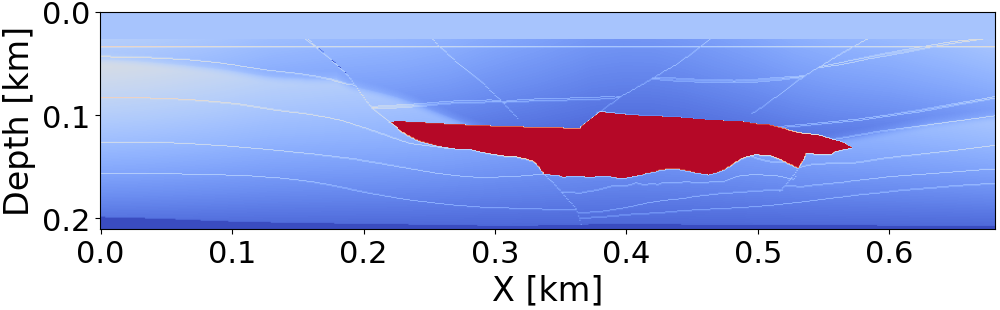
\includegraphics[width=80mm]{public/full_true_vm} &
        \raisebox{1.5mm}{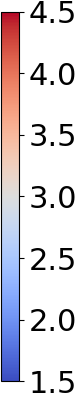
\includegraphics[height=23mm]{public/color-bar}}
    \end{tabular}
    \vspace{-2mm}
    \caption{The velocity model of the Salt [km/s]}
    \vspace{-2mm}
    \label{fig:salt-model}
\end{figure}


We introduce the TV and box constraint into the FWI problem to achieve more accurate reconstruction.
As shown in Fig.~\ref{fig:salt-model}, the velocity model is piecewise smooth, thus introducing the TV constraint to achieve a more accurate reconstruction.
The box constraint ensures that the velocity model remains within valid ranges.

The optimization problem of the TV and box constrained FWI is formulated as follows:
\begin{equation} \label{eq:FWIObjectiveWithTVConstraint} \argmin{\velModel \in \realNumber^N} \ \ \FWIObjectiveWithTVConstraint \end{equation}
where $\alpha \in \realNumber$ is the upper bound of the $l_{1,2}$ norm, and $l, u \in \realNumber$ are the lower and upper bounds of the velocity model values, respectively.
By incorporating TV as a constraint, the parameter $\alpha$ can be determined independently of other terms or constraints, which has been highlighted as an advantage in prior works~\cite{constraint0,constraint1,constraint2,constraint3,constraint4,constraints-vs-penalties-in-FWI}.
This separation makes it possible to directly control smoothness according to $\alpha$, providing a clearer interpretation of the reconstructed subsurface properties.

The constraints can be incorporated into the objective function as indicator functions:
\begin{equation} \label{eq:FWIObjectiveWithTVConstraintWithIndicatorFunction} \argmin{\velModel \in \realNumber^N} \ \ \FWIObjectiveWithTVConstraintWithIndicatorFunction, \end{equation}
where
\begin{equation} \label{eq:LOneTwoBallDefinition} \begin{aligned} \BoxBall & \coloneqq [l,u]^N, \\ \LOneTwoBall & \coloneqq \LOneTwoBallSetDefinition. \end{aligned} \end{equation}


The proximity operator of $\iota_{\BoxBall}$ and $\iota_{\LOneTwoBall}$ can be computed efficiently.
Therefore, these functions of $E$, $\iota_{\BoxBall}$ and $\iota_{\LOneTwoBall}$ correspond to $f$, $g$ and $h$ in \eqref{eq:PDSPrimalEq}, respectively, $\diffOperator$ is corresponds to $\bm{L}$, so the problem~\eqref{eq:FWIObjectiveWithTVConstraintWithIndicatorFunction} can be solved using PDS.
We show the detailed algorithm in Algorithm~\ref{alg:FWIWithPDS}.
%\begin{equation} \label{eq:FWIWithPDS} \FWIWithPDS \notag \end{equation}
\begin{algorithm}[t]
    \caption{PDS for \eqref{eq:FWIObjectiveWithTVConstraintWithIndicatorFunction}}\label{alg:FWIWithPDS}
    \begin{algorithmic}[1]
        \Statex \textbf{Input:} $ \velModel^{(0)}, \vecy^{(0)}, \gamma_0 > 0, \gamma_1 > 0 $
        \While {A stopping criterion is not satisfied}
            \State $\widetilde{\velModel} \leftarrow \FWIWithPDSStepMTmp $
            \State $\velModel^{(k+1)}     \leftarrow \FWIWithPDSStepM $
            \State $\widetilde{\vecy}     \leftarrow \FWIWithPDSStepYTmp $
            \State $\vecy^{(k+1)}         \leftarrow \FWIWithPDSStepY $
        \EndWhile
        \Statex \textbf{Output:} $\velModel^{(k)}$
    \end{algorithmic}
\end{algorithm}


The proximity operators of $\iota_{\BoxBall}$, $\iota_{\LOneTwoBall}$, that is, the projection onto $\BoxBall$ and ${\LOneTwoBall}$ are calculated by
\begin{equation} \label{eq:ProximityOperatorForBoxConstraint} \projBoxSolution, \end{equation}
\begin{equation} \label{eq:ProximityOperatorForL12Ball} \projLOneTwoBallSolution \end{equation}
where
\begin{equation} \label{eq:ProximityOperatorForL12BallWhere} \projLOneTwoBallSolutionWhere, \end{equation}
and $\mathfrak{g}_i$ is an index set corresponding to the horizontal and vertical differences of the $i$-th element of $\velModel$.

The proximity operator for the $l_1$ norm upper bound constraint is expressed as follows~\cite{L1-ball-projection}:
\begin{equation} \label{eq:ProximityOperatorForL1Ball}  \projLOneBallSolution, \end{equation}
where
\begin{equation} \label{eq:ProximityOperatorForL1BallWhere} \projLOneBallSolutionWhere \end{equation}

Our algorithm can incorporate the constraints without requiring any approximations.
Furthermore, since our algorithm can solve the TV and box constrained FWI problem without inner loops, it can be executed efficiently.
In fact, the incorporation of the constraints does not significantly increase the overall computational cost, because it is fast enough compared to the $\nabla E$ computation, which requires simulation of the wave equation along the time axis.
